\scanpage{14}
% archive sheet number: 13
\[
\begin{aligned}
 \Gamma_1&:\Gamma'_2\cup\Gamma'_3\\
 \Gamma_2&=\Gamma'_3\cup\Gamma'_1\\
 \Gamma_3&:\Gamma'_1\cup\Gamma'_2
\end{aligned}
\]

\diagram{\begin{tikzcd}[ampersand replacement=\&,column sep=small,row sep=small,font=\small]
 \& {\begin{gathered}\mathrm{a)}\quad\unsure{v|\nu}_1,v_2,v_3\\
 \text{\deleted{\unsure{appartiennent|appartenant}}\inserted{contenus} dans}\\
 \text{régions distinctes}\\[-2pt]\text{de }E-\Gamma\end{gathered}}
 \arrow[d,Rightarrow] \\
 {\begin{gathered}\mathrm{a}')\ E-\Gamma\text{ a}\\
 \text{trois régions}\\\text{distinctes}\end{gathered}}\arrow[ur,Leftrightarrow]
 \& {\begin{gathered}\mathrm{b)}\quad\Gamma_1,\Gamma_2,\Gamma_3\text{ sont des courbes de}\\
 \text{Jordan}\end{gathered}}\arrow[d,Rightarrow]\\
 \&{\begin{gathered}\mathrm{c)}\quad\Gamma_1,\Gamma_2\text{ sont des courbes}\\
 \text{de Jordan}\end{gathered}}
\end{tikzcd}}

\figure{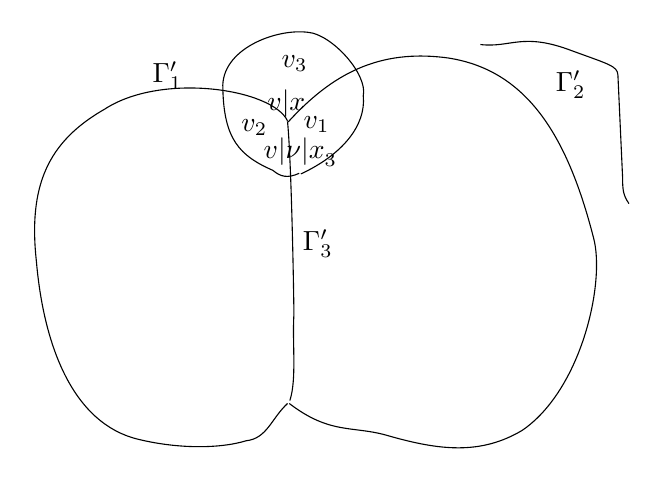
\begin{tikzpicture}[x=0.74cm,y=0.74cm]
\draw (4.34,5.59) .. controls (4.08,6.14) and (2.18,6.43) .. (1.20,5.79)
 .. controls (0.22,5.23) and (-0.11,4.47) .. (0.03,3.18)
 .. controls (0.16,1.68) and (0.68,0.40) .. (1.76,0.13)
 .. controls (2.44,-0.04) and (3.17,-0.04) .. (3.63,0.10)
 .. controls (3.99,0.14) and (4.06,0.48) .. (4.34,0.74);
\draw (4.35,5.57) .. controls (5.10,6.39) and (5.90,6.83) .. (7.09,6.67)
 .. controls (8.49,6.46) and (9.16,5.26) .. (9.59,3.59)
 .. controls (9.80,2.83) and (9.39,0.98) .. (8.37,0.28)
 .. controls (7.65,-0.15) and (6.94,-0.06) .. (6.09,0.18)
 .. controls (5.47,0.37) and (5.09,0.19) .. (4.37,0.74);
\draw (4.34,5.58) .. controls (4.40,4.97) and (4.44,3.09) .. (4.45,2.28)
 .. controls (4.42,1.76) and (4.50,1.16) .. (4.38,0.79);
\draw (4.57,4.68) .. controls (5.28,5.01) and (5.69,5.51) .. (5.64,6.02)
 .. controls (5.72,6.40) and (5.09,7.08) .. (4.69,7.11)
 .. controls (4.14,7.18) and (3.19,6.82) .. (3.23,6.14)
 .. controls (3.25,5.27) and (3.52,4.99) .. (4.09,4.74)
 .. controls (4.22,4.63) and (4.34,4.60) .. (4.54,4.69);
\draw (7.65,6.90) .. controls (8.18,6.84) and (8.37,7.12) .. (9.23,6.79)
 .. controls (9.86,6.56) and (10.00,6.53) .. (10.01,6.38)
 --(10.09,4.63) .. controls (10.09,4.41) and (10.10,4.31) .. (10.20,4.17);
\node at (2.28,6.36) {$\Gamma'_1$};
\node at (9.20,6.21) {$\Gamma'_2$}; \node at (4.86,3.48) {$\Gamma'_3$};
\node at (4.46,6.58) {$v_3$}; \node at (3.77,5.47) {$v_2$};
\node at (4.84,5.52) {$v_1$}; \node at (4.32,5.88) {$\deleted{\unsure{v|x}}$};
\node at (4.56,5.05) {$\deleted{\unsure{v|\nu|x}_3}$};
\end{tikzpicture}}

\[
\begin{aligned}
 &\mathrm{a)}\unsure{\Longleftrightarrow|\longleftrightarrow}\mathrm{a}')\\
 &\mathrm{b)}\Longrightarrow\mathrm{c)}\deleted{\unsure{\Rightarrow|\Leftrightarrow}}\ \text{triv}\\
 &\mathrm{c)}\Longrightarrow\mathrm{a)}
\end{aligned}
\]

\deleted{\unsure{En suivant|En traversant|En entourant} $\Gamma'_3$ \unsure{on dit|on doit}}
Car 2 pts de part et d'\deleted{\unsure{autre|sont|au}}autre de $\Gamma'_3$ \unsure{doivent|disons}
\unsure{être} ds des régions distinctes de $E-\Gamma_1$
(\inserted{\unsure{ou}} $E-\Gamma_2$), \unsure{en|sont} \inserted{a fortiori} \unsure{plus|alors|des} régions distinctes de
\deleted{\inserted{$\unsure{E'|E}$}$E-\unsure{\Gamma_1\cup\Gamma_2|\Gamma_1\cap\Gamma_2|\Gamma_2}$}
\inserted{$=E-\Gamma$}, donc $v_1$ et $v_2$ sont \unsure{dans|des} régions distinctes.
\unsure{De|D} $=$, deux pts de part et d'autre de $\Gamma'_1$ \inserted{($\Gamma'_2$)}
sont \unsure{dans|des} régions distinctes de $E-\Gamma_2$ ($E-\Gamma_1$) donc sont \unsure{dans|des} régions distinctes
dans $E-\Gamma$, OK.

$\mathrm{a)}\Longrightarrow\mathrm{b)}$\qquad Prouvons que $\Gamma_3$ (p.ex.) est courbe de Jordan.
